\section{Data}
\label{sec:data}

Training a generalist vision-language-action model requires data that is
simultaneously large in scale, diverse across embodiments, tasks, and scenes,
and high in quality. The robotics community has released several substantial
public corpora toward this goal---most notably the Open X-Embodiment (OXE)
mixture~\citep{o2024open}, DROID~\citep{khazatsky2024droid}, and a rapidly
growing collection of LeRobot community datasets contributed by
SO-10x users~\citep{shukor2025smolvlavisionlanguageactionmodelaffordable}. While each is valuable, none of these
resources individually, nor their union, is sufficient for training a model
intended for real-world deployment. OXE offers breadth across embodiments
but its constituent datasets vary widely in quality, control conventions,
and language-annotation fidelity; DROID provides scale on a single Franka
platform, but a substantial fraction of its episodes contain idle segments,
failed attempts, or repetitive task instructions; and crowd-sourced LeRobot
data, although rich in embodiment and scene diversity, frequently contains
placeholder annotations such as ``lerobot\_test'' alongside genuine
demonstrations~\citep{shukor2025smolvlavisionlanguageactionmodelaffordable}.
Critically, no public corpus contains high-quality bimanual manipulation
data on the platform we target for deployment, and the tasks that are
covered are often collected with limited variation in scene configuration,
object instances, or spatial variation that mimic the realistic of real-world tasks for deployment.

To close these gaps, we assemble \molmoactt's training mixture from three
complementary sources, summarized in Fig.~\ref{yamsetup}. First, we collect
\molmoacttyamdata, a new bimanual manipulation dataset emphasizing task
repeatability and task, object, and scene diversity across a wide range of
useful behaviors. Second, we curate and filter two large public corpora,
\molmoacttsodata (drawn from community LeRobot data) and \molmoacttdroiddata
(drawn from DROID), using structural, licensing, and quality-based
filtering pipelines, and re-annotate their language instructions to improve
both accuracy and diversity. Third, we co-train with a targeted subset of
academic robotics data for additional embodiment breadth, together with
multimodal and embodied-reasoning data to preserve the broad visual and
linguistic competence of the underlying VLM. The remainder of this section
describes each component of the mixture in turn, together with the language
re-annotation pipeline shared across our robot datasets.

\begin{figure}[t]
    \centering
    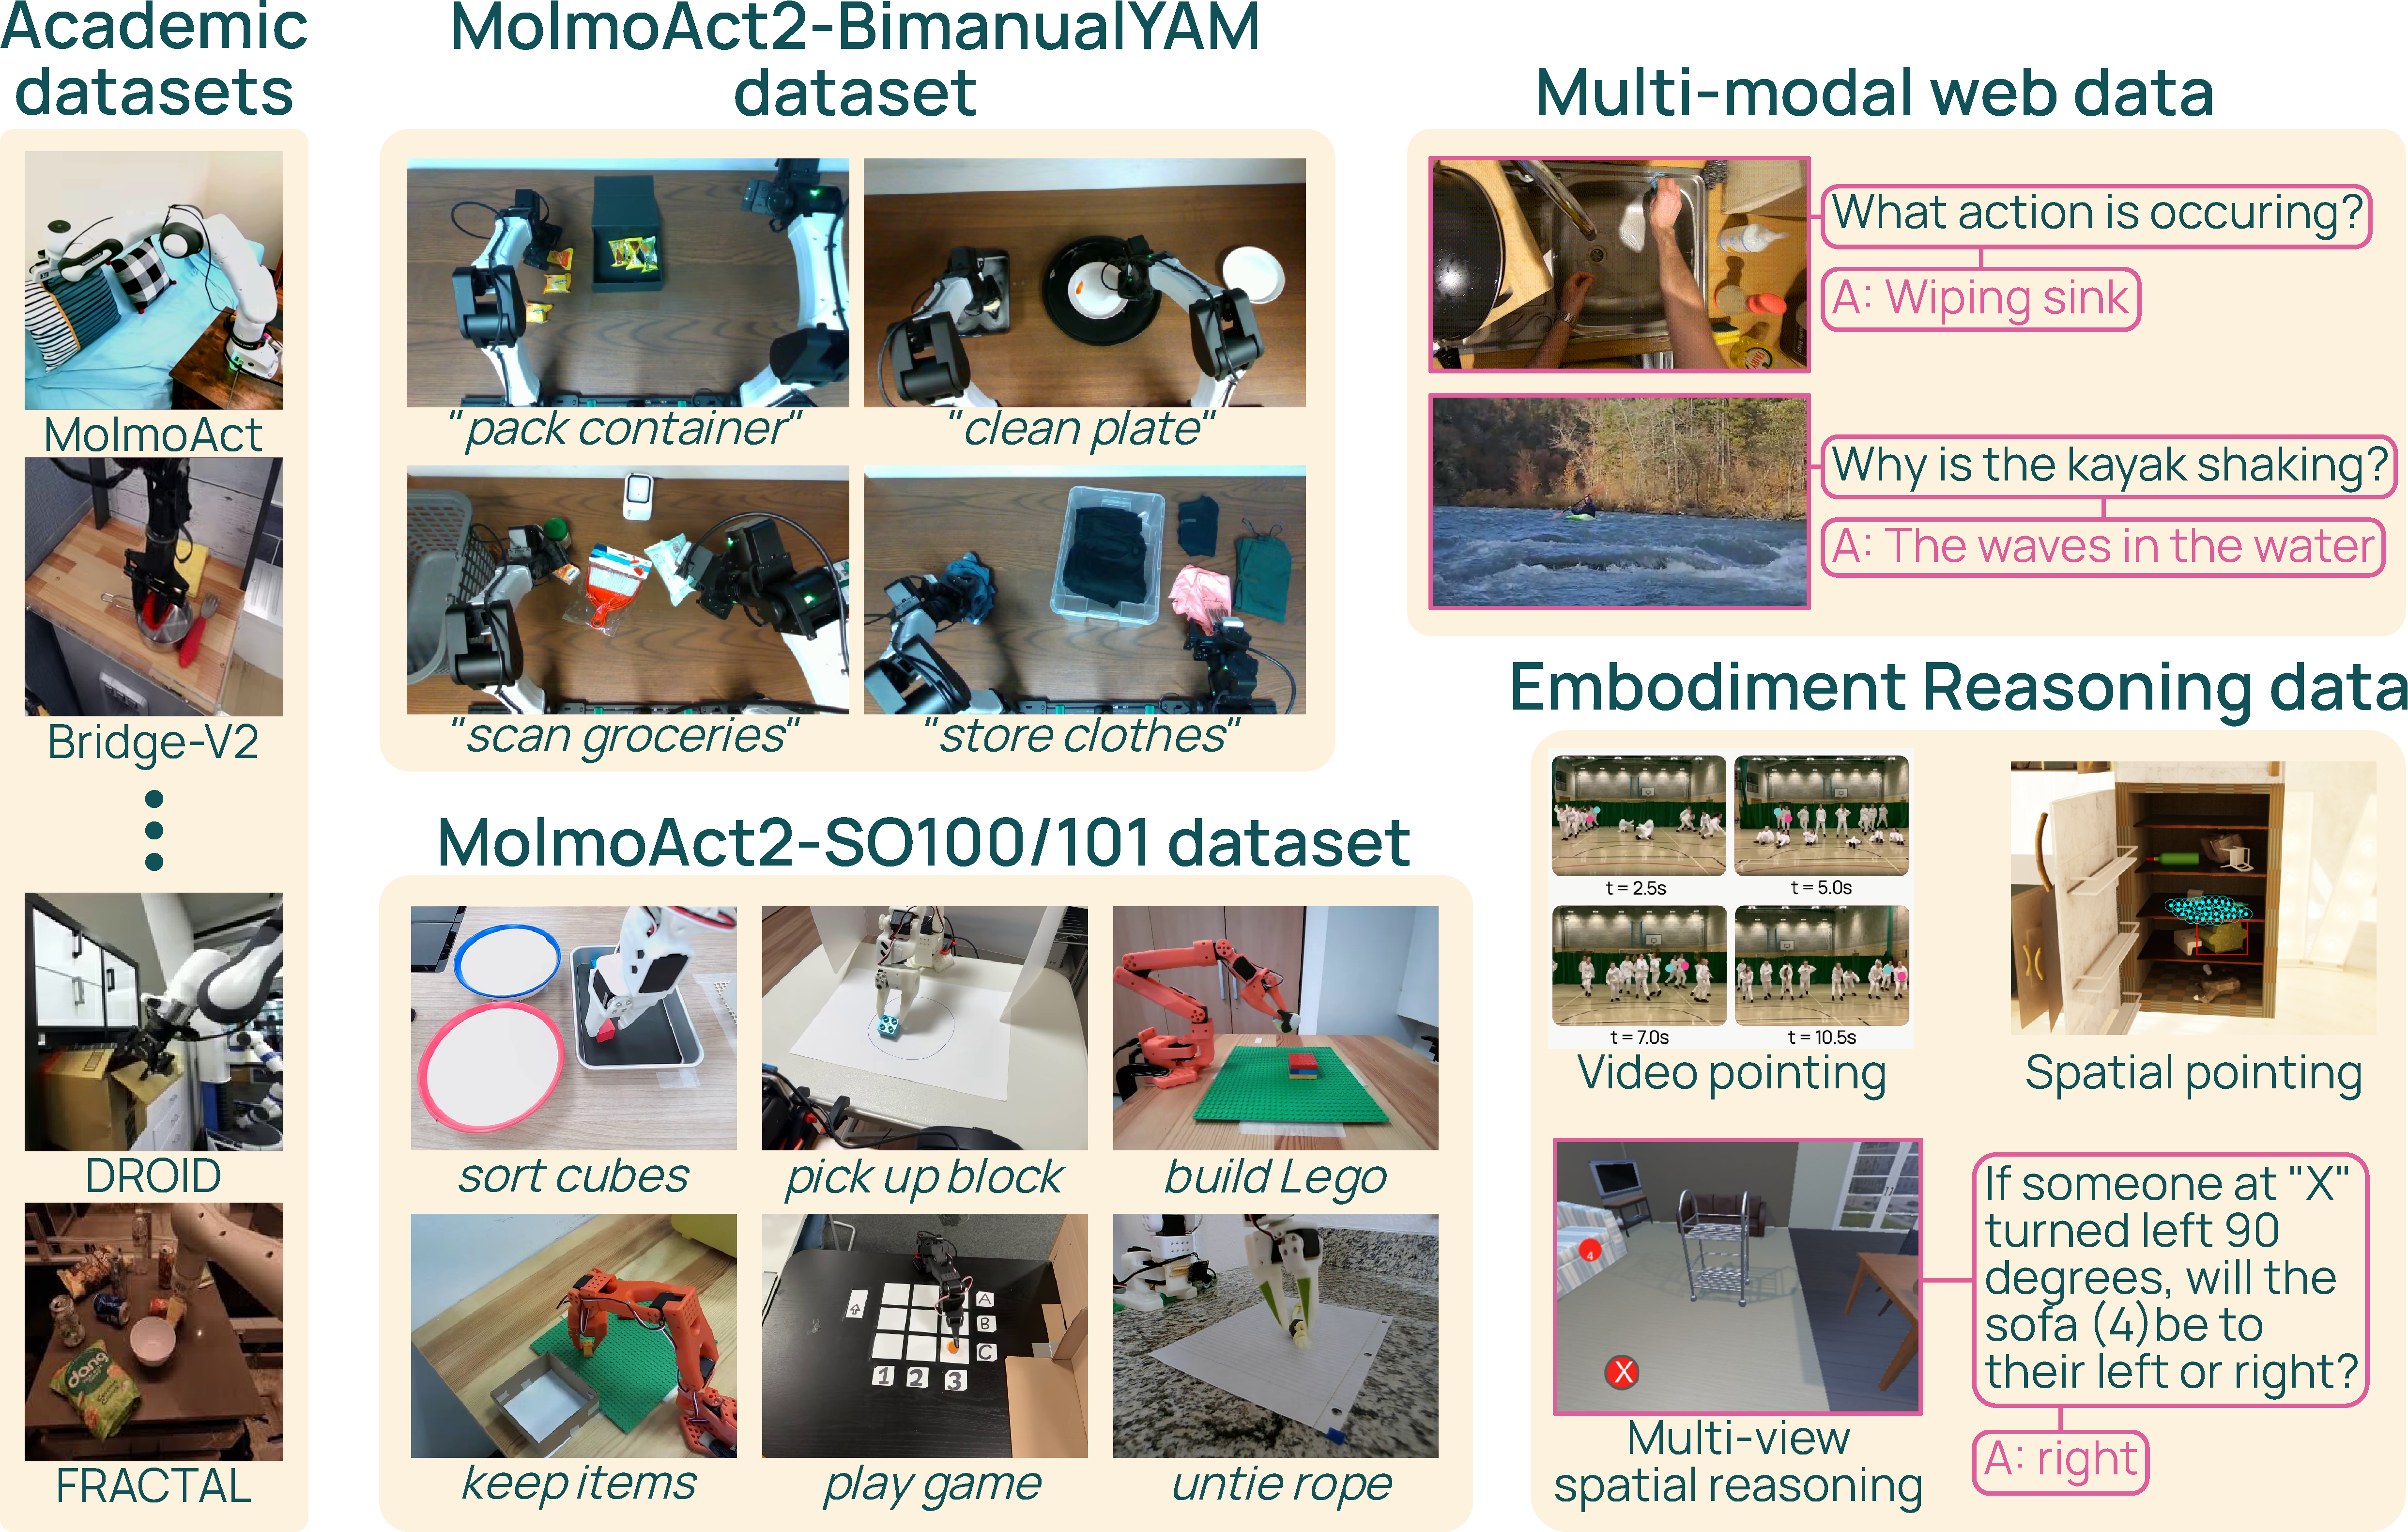
\includegraphics[width=\linewidth]{figures/Data_4.pdf}
    \caption{\textbf{Overview of the \molmoactt training data.} Our data mixture combines public academic robot datasets, \molmoacttyamdata, \molmoacttdroiddata, \molmoacttsodata, multimodal web data, and embodied-reasoning data.}
    \label{yamsetup}
\end{figure}

% \ranjay{Let's start off by talking about why there was a need for more data. Lay out what data is available publicly and why it is not enough.}

\molmoactt is trained on a diverse set of datasets spanning robot data, multimodal reasoning, and embodied reasoning, summarized in Fig.~\ref{yamsetup}. Additionally, we collected \molmoacttyamdata, curated \molmoacttsodata, and filtered \molmoacttdroiddata for use in pre-training and post-training. Below, we describe each dataset and detail its respective collection, curation, or filtering process.


\subsection{\molmoacttyamdata}
To support real-world deployment, we introduce \molmoacttyamdata, an open-source robot manipulation dataset that emphasizes task repeatability, task diversity, and object diversity across a broad range of useful behaviors spanning household, factory, and coffee-shop settings. All data is collected on our custom bimanual YAM (Yet Another Manipulator) setup, shown in Figure~\ref{fig:dataset-setup}. \molmoacttyamdata is designed to deliver both scale and quality. It contains over 28 unique real-world tasks from folding clothes and untangling cables to bussing tables, scanning groceries, and packing medication, each captured with substantial variation in scene configuration, object instances, and object placement. In total, the dataset comprises 34.5k robot demonstrations totaling over 720 hours of robot data, collected over a two-month period. Data collection was supported by Cortex AI, with strict protocols governing the number of permitted failure retries and the maximum duration of no-op segments to ensure consistently high data quality. Further details on \molmoacttyamdata are provided in the appendix.

\subsection{\molmoacttsodata}
\label{sec:so100-dataset}
SO-100/101 is a low-cost robotic platform from Hugging Face that is accessible to a broad community of users. As a result, we utilize the diverse open-source SO-10x data collected by the community to improve our model's capability for deployment in the wild \citep{chen2025depi}. Specifically, we curate \molmoacttsodata from 1{,}222 public LeRobot datasets contributed by 377 users. This corpus contains 38{,}059 robot demonstration episodes, 19.8M frames, and approximately 184 hours of interaction data.

To prioritize quality while preserving diversity, we apply a four-stage filtering pipeline: (i) structural validity checks (required schema fields, valid action/state tensors, no NaN/corrupt samples), (ii) removal of eval-style datasets, (iii) license/codebase eligibility checks, and (iv) a final TOPReward quality gate ~\citep{chen2026topreward}. In stage (iv), we keep datasets whose mean TOPReward over the last 3 sampled episodes is above a threshold obtained by averaging the TOPReward over a collection of human-audited high-quality datasets.


\begin{figure}[t]
    \centering
    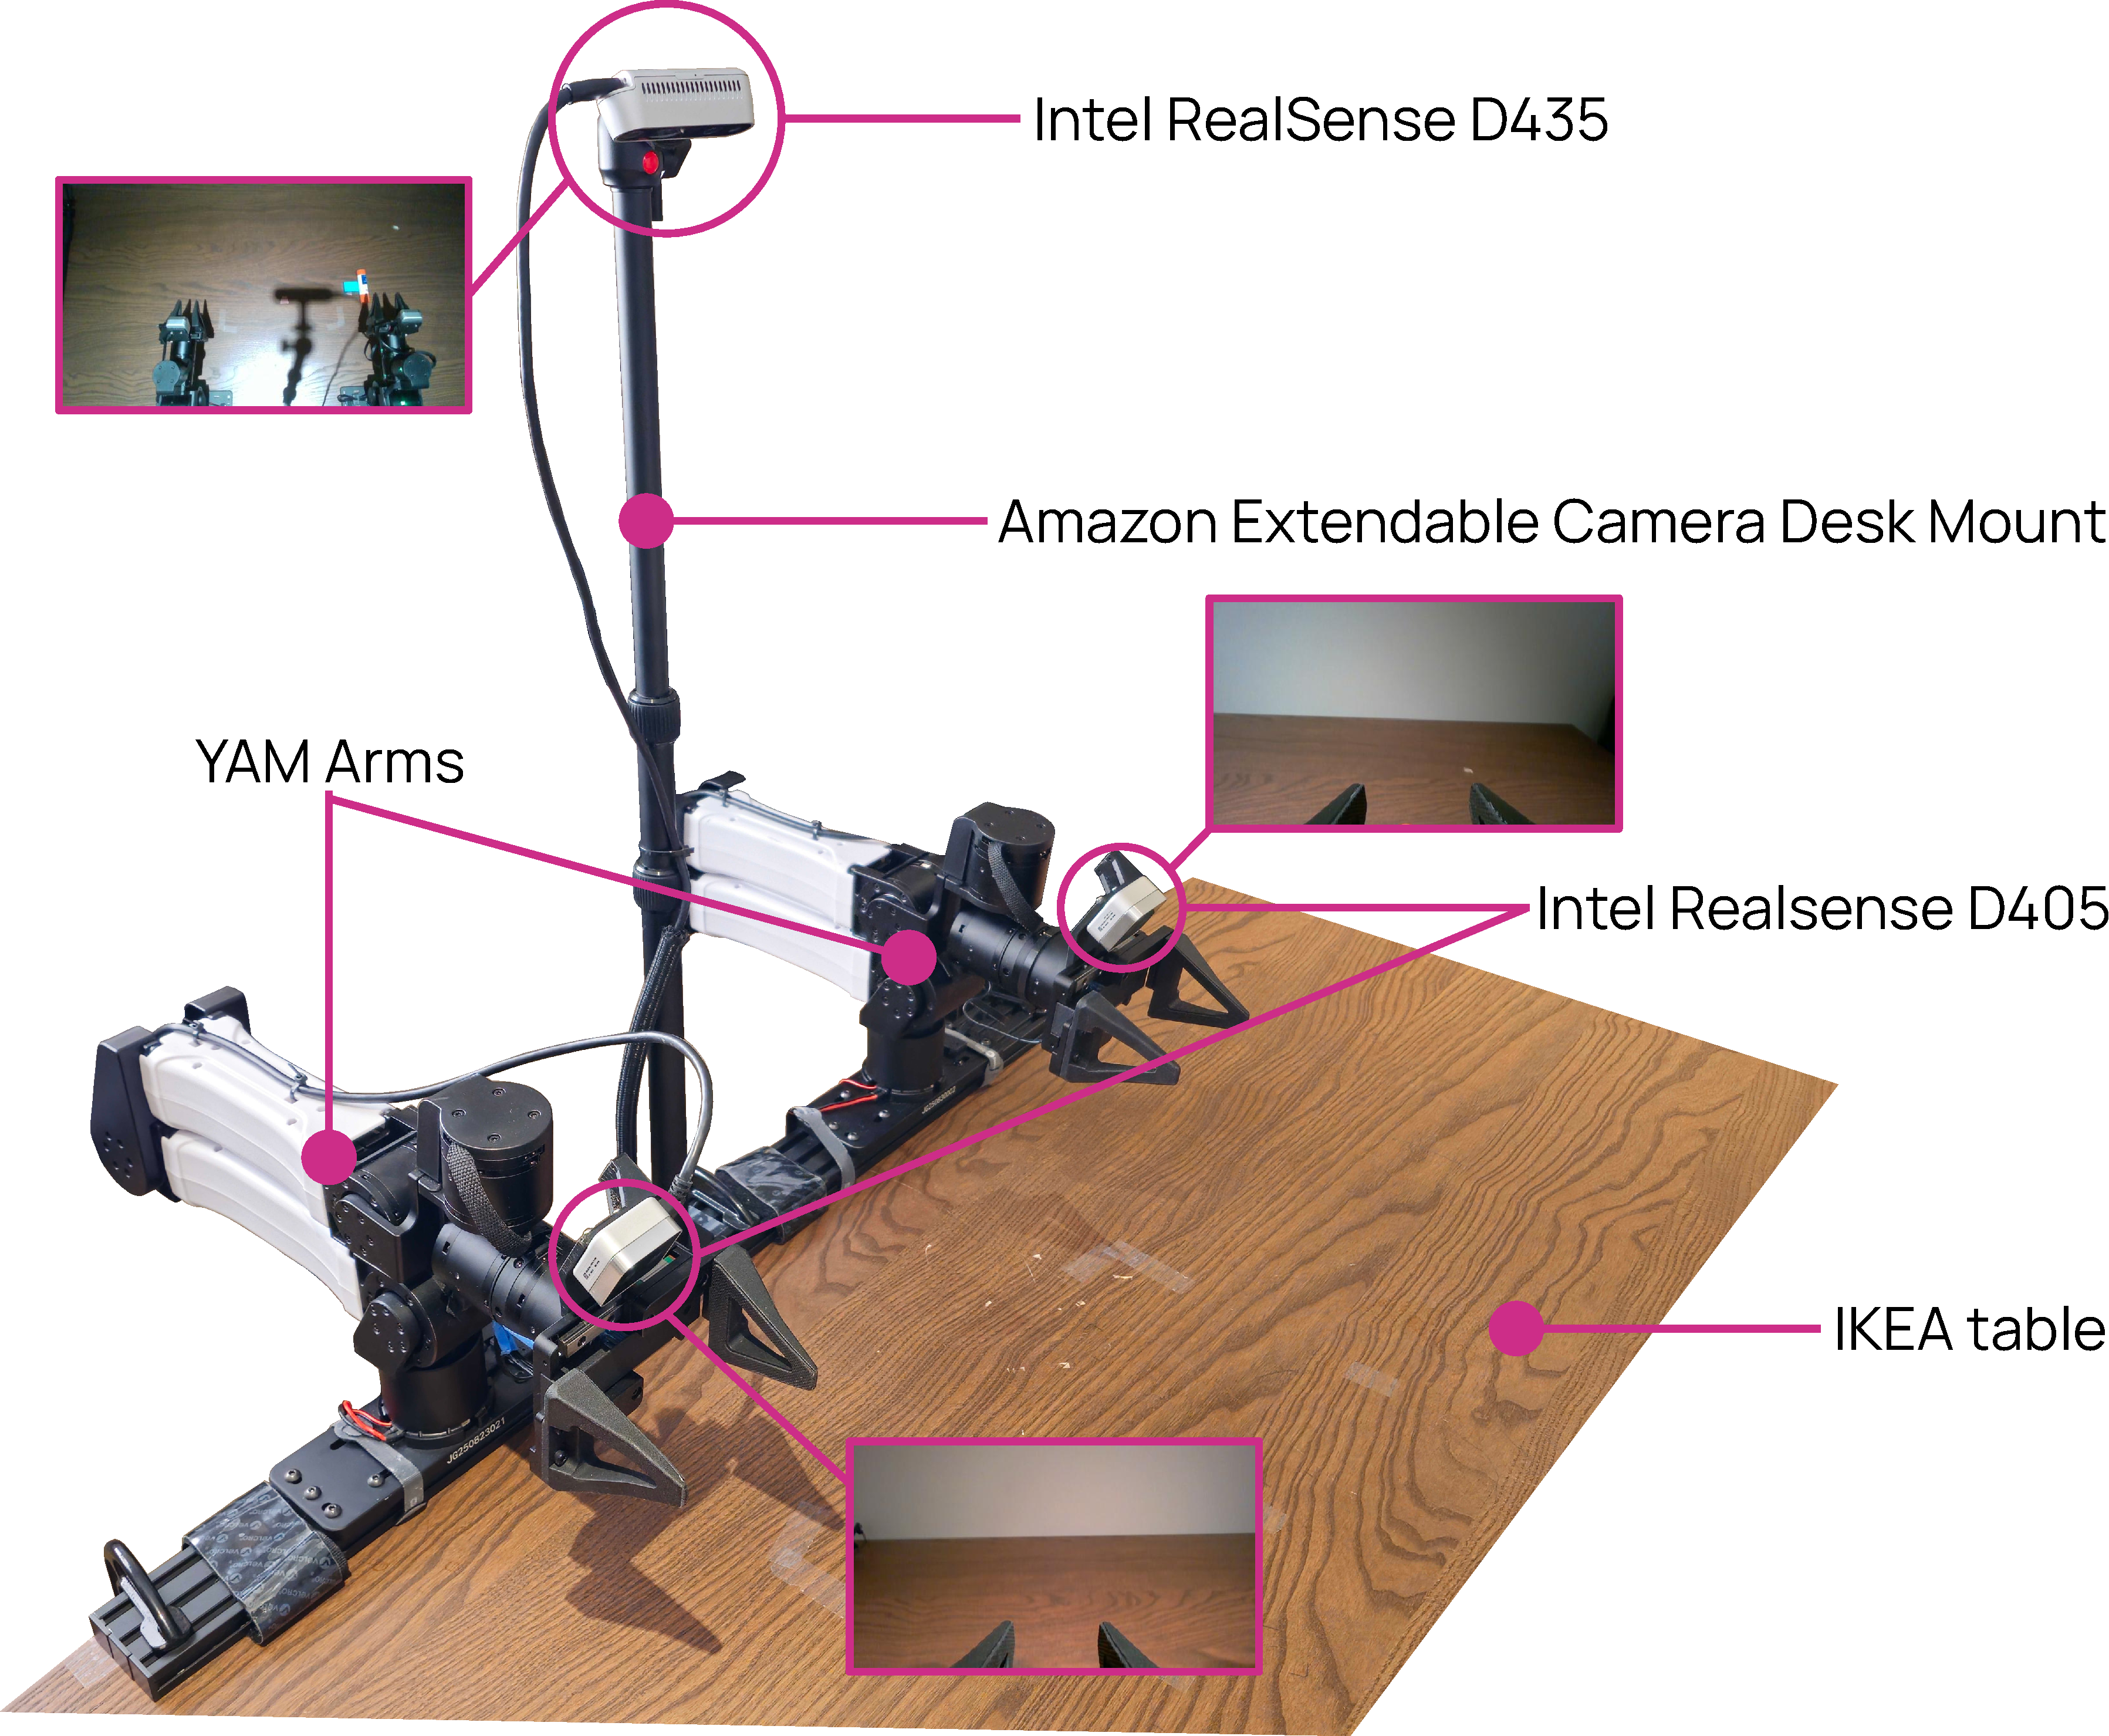
\includegraphics[width=0.6\linewidth]{figures/Setup2.pdf}
    \caption{\textbf{\molmoacttyamdata collection setup.}
Our standardized \molmoacttyamdata collection setup. Every component is readily
available for purchase, and the total cost of the entire setup is under \$6{,}000 USD.}
    \label{fig:dataset-setup}
\end{figure}

The filtered data spans both SO-100 and SO-101 embodiments, multiple camera configurations, varied object manipulation tasks, and diverse real-world collection environments. Compared with centrally collected robot datasets, this community-sourced corpus provides broader coverage of user setups, backgrounds, objects, and task annotations, making it a useful source of embodiment and environment diversity for improving real-world robustness.

\subsection{\molmoacttdroiddata}
DROID (Distributed Robot Interaction Dataset)~\citep{khazatsky2024droid} is a large-scale in-the-wild robot manipulation dataset, collected across a wide range of real-world deployment scenarios with a unified Franka robot setup. To ensure the quality of our training data, we leverage the supplementary annotations released in the accompanying HuggingFace repository~\citep{pertsch2024droidannotations} to filter the original DROID release. Specifically, we use (i) the extended language annotations, which provide three natural-language instructions for 95\% of the 75k successful episodes, and (ii) the provided idle-frame filter, which retains only contiguous non-idle action segments of at least one second. Furthermore, we did language re-annotation for the filtered DROID dataset before using for training. The resulting subset, which we refer to as \molmoacttdroiddata, contains 74,604 valid episodes comprising a total of 17{,}758{,}044 frames. Each episode in this subset is marked as successful, contains at least one valid language instruction, and is free of significant pauses. 



\subsection{Language annotation pipeline}
\label{sec:lang_annot}
Following standard practice in imitation learning, each demonstration in our datasets is paired with a language instruction that describes the task completed by the teleoperator. However, we find that these annotations often are imperfect along two key axes. First, datasets where a specific set of tasks is collected repeatedly at scale often have repetitive language instructions. For example, the dataset collected in \cite{jang2022bc} contains 104 unique instructions for 39350 episodes, representing $0.26\%$ unique instructions in the dataset. Secondly, as found in prior work \citep{shukor2025smolvlavisionlanguageactionmodelaffordable}, crowd-sourced datasets like the \molmoacttsodata often have inaccurate or meaningless task annotations, like "lerobot\_test" and "Test run".

To improve both the diversity and accuracy of the language instructions in our robotics datasets, we use an open-source VLM (Qwen3.5-27B) to re-annotate the datasets. We prompt the VLM with a sample of the frames and the original instruction. The VLM is asked to generate a instruction that describes the demonstration. To increase the diversity of prompts, we randomly sample a number and ask the VLM to make this instruction roughly that many words. Relabeling the robotics datasets through this pipeline doubles the unique labels in the overall from 71121 (22\%) to 146485 (46\%) in dataset. More details and the prompt can be found in Appendix \ref{supp:language-annotation-details}.


\subsection{Academic robotics datasets}
% Beyond our main deployment datasets, we include additional public academic robotics data to broaden the range of embodiments, camera layouts, task families, and control conventions seen during pre-training. 
To broaden the range of embodiments, camera layouts, task families, and control conventions seen during pre-training, we include additional public academic robotics data. This pool consists of a targeted subset of the Open X-Embodiment mixture~\citep{o2024open}, including BC-Z~\citep{jang2022bc}, BridgeData V2~\citep{walke2023bridgedata},
and RT-1~\citep{brohan2022rt}, together with \molmoactdata from \molmoact~\citep{lee2025molmoactactionreasoningmodels}. These datasets are used as complementary sources rather than as the primary deployment embodiments, since YAM, SO-100/101, and DROID supply the majority of robot training examples.

\subsection{Multimodal datasets}
Past research on robotics foundation models has found benefits in incorporating multimodal data into the training mix along with robotics datasets \citep{lee2025molmoactactionreasoningmodels, intelligence2025pi05visionlanguageactionmodelopenworld}. We co-train the VLA with a multimodal data mixture where 46\% consists of the \molmoer dataset mixture described in Sec.~\ref{sec:molmoer-data}, 46\% consists of the \molmot dataset mixture~\citep{clark2026molmo2openweightsdata}, and 8\% consists of the text-only data from Tulu-3 ~\citep{lambert2025tulu3pushingfrontiers}. The high level composition of this data can be seen in Table \ref{tab:molmoact2-vqa-data}.

% The Image QA bucket consists of multiple choice and short answer questions on images. The Video QA bucket also consists of multiple choice and short answer questions, but on video datasets. The Image Pointing bucket consists of points on images that correspond to the description in the text. The Video Pointing bucket consists of point and description pairs but for a subset of a video's frames. The Video Tracking bucket consists of tracks, such as point, segmentation, and bounding boxes around the described object in the video clip. The Captions/LongQA bucket consists of various long form question answer pairs for images and videos.


